% Gemini theme
% https://github.com/anishathalye/gemini

\documentclass[final]{beamer}

% ====================
% Packages
% ====================

\usepackage[T1]{fontenc}
\usepackage{lmodern}
% \usepackage[size=custom,width=120,height=72,scale=1.0]{beamerposter}
\usepackage[size=custom,width=121.92,height=91.44,scale=1.0]{beamerposter}
\usetheme{cml}
\usecolortheme{cml}
\usepackage{graphicx}
\usepackage{booktabs}
\usepackage{tikz}
\usepackage{pgfplots}
\pgfplotsset{compat=1.14}
\usepackage{anyfontsize}
\usepackage{svg}
\usepackage[acronym,nohypertypes={acronym,notation}]{glossaries}
\glsdisablehyper
\newacronym{dnn}{DNN}{Deep Neural Network}
\newacronym{cnn}{CNN}{Convolutional Neural Network}
\newacronym{nn}{NN}{Neural Network}
\newacronym{ann}{ANN}{Artificial Neural Network}
\newacronym{snn}{SNN}{Sparse Neural Network}
\newacronym{lt}{LT}{Lottery Ticket}
\newacronym{ntk}{NTK}{the Neural Tangent Kernel}
\newacronym{lth}{LTH}{Lottery Ticket Hypothesis}
\newacronym{nlp}{NLP}{Natural Language Processing}
\newacronym{dst}{DST}{Dynamic Sparse Training}
\newacronym{gpu}{GPU}{Graphics Processing Unit}
\newacronym{pi}{PI}{Primary Investigator}
\newacronym{ai}{AI}{Artificial Intelligence}
\newacronym{ml}{ML}{Machine Learning}
\newacronym{cv}{CV}{Computer Vision}
\newacronym{neurips}{NeurIPS}{Neural Information Processing Systems}
\newacronym{iclr}{ICLR}{the International Conference on Learning Representations}
\newacronym{cvpr}{CVPR}{the IEEE/CVF Conference on Computer Vision and Pattern Recognition}
\newacronym{flops}{FLOPs}{Floating Point Operations}
\newacronym{relu}{ReLU}{ReLU}
\newacronym{srigl}{SRigL}{Structured RigL}
\newacronym{rigl}{RigL}{Rigging the Lottery Ticket}
\newacronym{set}{SET}{Sparse Evolutionary Training}
\newacronym{erk}{ERK}{Erd\H{o}s-R\'enyi-Kernel}
\newacronym{ste}{STE}{Straight-Through Estimator}
\newacronym{srste}{SR-STE}{Sparse-Refined Straight-Through Estimator}
\newacronym{ilsvrc}{ILSVRC-12}{2012 ImageNet Large Scale Visual Recognition Challenge}
\newacronym{ast}{AST}{Alternating Sparse Training}
\newacronym{deepr}{DeepR}{Deep Rewiring}
\newacronym{snfs}{SNFS}{Sparse Networks from Scratch}
\newacronym{dsr}{DSR}{Dynamic Sparse Reparameterization}
\newacronym{topkast}{Top-KAST}{Top-K Always Sparse Training}
\newacronym{mest}{MEST}{Memory-Economic Sparse Training}
\newacronym{dsb}{DSB}{Dynamic Shuffled Block}
\newacronym{dynsparse}{DynSparse}{Dynamic Sparsity}
\newacronym{vit}{ViT-B/16}{Vision Transformer}
\newacronym{cpu}{CPU}{Central Processing Unit}
\glsunset{rigl} % We don't like to expand the RigL acronym
\usepackage[numbers,sort]{natbib}
\usepackage{threeparttable} % To use tables with footnotes properly
\usepackage[font=small,labelfont=bf,tableposition=top]{caption}
% % Reset all the acronyms/glossary for main paper
% \glsresetall

% ====================
% Lengths
% ====================

% If you have N columns, choose \sepwidth and \colwidth such that
% (N+1)*\sepwidth + N*\colwidth = \paperwidth
\newlength{\sepwidth}
\newlength{\colwidth}
% 3 cols
\setlength{\sepwidth}{0.025\paperwidth}
\setlength{\colwidth}{0.3\paperwidth}

% 2 cols
% \setlength{\sepwidth}{0.025\paperwidth}
% \setlength{\colwidth}{0.475\paperwidth}

\newcommand{\separatorcolumn}{\begin{column}{\sepwidth}\end{column}}

% ====================
% Title
% ====================

\title{Dynamic Sparse Training with Structured Sparsity}
\author{
    Mike Lasby$^{1}$,
    Anna Golubeva$^{2,3}$,
    Utku Evci$^{4}$,
    Mihai Nica$^{5,6}$,
    Yani A.\ Ioannou$^{1}$
}

\institute[shortinst]{
    $^{1}$University of Calgary \samelineand
    $^{2}$Massachusetts Institute of Technology \samelineand
    $^{3}$IAIFI \samelineand
    $^{4}$Google Research \samelineand
    $^5$University of Guelph \samelineand
    $^6$Vector Institute for AI
}


% ====================
% Footer (optional)
% ====================

\footercontent{
  \RaggedLeft
  \large
  Arxiv: 
  \begin{array}{l}
    \includesvg[height=3.5cm]{qr/srigl-arxiv-qr.svg}
  \end{array}
  \hfill
  \centering
  Upper Bound $2023$ --- Edmonton, AB
  \hfill
  \RaggedRight
  CalgaryML Lab:
  \begin{array}{l}
    \includesvg[height=3.5cm]{qr/calgaryml-qr.svg}
  \end{array}
}
% (can be left out to remove footer)

% ====================
% Logo (optional)
% ====================

% use this to include logos on the left and/or right side of the header:
% White Logos

\newlength{\logooffset}
\setlength{\logooffset}{2ex}
\newlength{\logoheight}
\setlength{\logoheight}{3.5cm}
% white logos
% \logoright{
%     \includegraphics[height=\logoheight]{iaifi-logo-white.pdf}
%     \hspace{\logooffset}
%     \includegraphics[height=\logoheight]{vector-white-logo.png}
%     \hspace{\logooffset}
%     \includesvg[height=\logoheight]{ucmllogo-text-all-white.svg}
%     \hspace{\logooffset}
%     \includesvg[height=\logoheight]{UC-horz-white.svg}
% }
% \logoleft{
%     \includesvg[height=\logoheight]{upper_bound.svg}
%     \hspace{\logooffset}
%     \includesvg[height=\logoheight]{University_of_Guelph_logo-white.svg}
%     \hspace{\logooffset}
%     \includesvg[height=\logoheight]{MIT_logo.svg}
%     \hspace{\logooffset}
%     \includesvg[height=\logoheight]{Google_2015_logo-white.svg}
% }

% Colour logos
\logoright{
    \includegraphics[height=\logoheight]{logos/iaifi-logo-black.pdf}
    \hspace{\logooffset}
    \includegraphics[height=\logoheight]{logos/Vector-Institute_Logo.png}
    \hspace{\logooffset}
    \includesvg[height=\logoheight]{logos/ucmllogo-text.svg}
    \hspace{\logooffset}
    \includesvg[height=\logoheight]{logos/UC-horz-rgb.svg}
}
\logoleft{
    \includesvg[height=\logoheight]{logos/upper_bound-black.svg}
    \hspace{\logooffset}
    \includesvg[height=\logoheight]{logos/University_of_Guelph_logo.svg}
    \hspace{\logooffset}
    \includesvg[height=\logoheight]{logos/MIT_logo-colour.svg}
    \hspace{\logooffset}
    \includesvg[height=\logoheight]{logos/Google_2015_logo.svg}
}


% ====================
% Body
% ====================
\setbeamertemplate{caption}[numbered]
\begin{document}

\begin{frame}[t]
\begin{columns}[t]
\separatorcolumn

\begin{column}{\colwidth}

  \begin{block}{Motivation}
  \heading{Unstructured \glspl{snn} are hard to accelerate!}
  % \textbf{\Large Unstructured \glspl{snn} are hard to accelerate}
  \begin{itemize}
      \item State-of-the-art \Gls{dst} methods learn \emph{unstructured} \glspl{snn} with 85--95\% fewer weights than dense models, while maintaining similar generalization.

      \item Sparse training methods employ sparsity \emph{both during training and inference}, unlike pruning and other methods~\citep{zhou2021learning} that only exploit sparsity at inference time.

      \item While unstructured \glspl{snn} enable a large reduction in \gls{flops} in theory, realizing these speedups on hardware is challenging. 
      \item Structured sparse pruning often results in worse generalization than unstructured \glspl{snn}.
  \end{itemize}
  \end{block}

  \begin{block}{Method}
  \begin{enumerate}
        % \item We propose a novel sparse-to-sparse \gls{dst} method, \gls{srigl}, based on \gls{rigl}~\citep{evci_rigging_2021}. \Gls{srigl} learns a \gls{snn} with constant fan-in structured sparsity while maintaining generalization comparable with \gls{rigl} up to a high sparsity level (99\%) for a variety of network architectures. This structure is a particular case of ``N:M sparsity'' which requires $N$ out of $M$ consecutive weights to be non-zero~\citep{NvidiaA100}.
        \item We propose a novel sparse-to-sparse \gls{dst} method, \gls{srigl}, based on \gls{rigl}~\citep{evci_rigging_2021}. \Gls{srigl} learns a \gls{snn} with constant fan-in structured sparsity while maintaining generalization comparable with \gls{rigl} up to a high sparsity level (99\%) for a variety of network architectures. This structure is a particular case of ``N:M sparsity''~\citep{NvidiaA100}.
        \item We show that at sparsity levels >90\% \gls{rigl} ablates whole neurons. By allowing ablation in \gls{srigl}, we match the generalization performance of \gls{rigl} even in this high-sparsity regime.
        \item We motivate our choice of structure with a theoretical analysis of \gls{snn} output norm variance and find that the constant fan-in constraint does not have a negative effect.
        \item We demonstrate that our constant fan-in sparsity enables a compact representation that is not only parameter- and memory-efficient, but also amenable to real-world acceleration.
    \end{enumerate}

    \begin{figure}
        \includegraphics[width=.85\colwidth]{srigl_example_figs/constantfanin.pdf}
        \caption{Constant fan-in pruning v.s.\ unstructured pruning.}\label{fig:constfanin}
    \end{figure}

    \end{block}

  \begin{block}{Constant Fan-In Theoretical Analysis}
  \begin{itemize}
      \item Smaller output variance is indicative of training stability
      % \item We derive exact expressions for the variance of the layer output norm at initialization for different sparsity types
      \item We derive exact expressions for the variance of the layer output norm at initialization
      \item Constant fan-in consistently yields smaller variance than other sparsity types
  \end{itemize}

\begin{figure}
    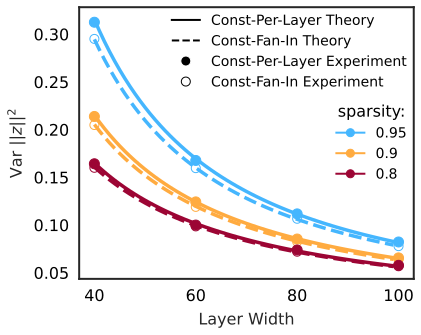
\includegraphics[width=.5\colwidth]{srigl_example_figs/Theory_1.pdf}
    % \includesvg[width=\colwidth]{fig/Theory_1.svg}
    \caption{Output-norm variance analysis.}\label{fig:theory}
\end{figure}
\end{block}

\end{column}
\separatorcolumn
\begin{column}{\colwidth}
  \begin{block}{Results}
  \begin{table}[p]
  \vspace{-1em}
    \begin{threeparttable}
    \begin{center}
        \caption{\textbf{Top-1 ImageNet test accuracy of ResNet-50 trained with a variety of \gls{dst} methods}, highlighting methods that both are sparse-to-sparse \emph{and} learn structured sparsity similar to \gls{srigl} --- only DSB-16 (2:4 and 1:4  sparsity) is directly comparable in this regard. \gls{rigl} and \gls{srigl} results are from our experiments, other values are obtained from each method's corresponding paper, U.N.O.}\label{table:imagenet_benchmarks}
        \begin{tabular}{@{}p{6.0em}p{4.0em}p{5.5em}cccccc@{}}\toprule
        & training &  & \multicolumn{5}{c}{sparsity} \\
        \cmidrule(lr){4-8}
         % \midrule
        method & method & structured & 50\% & 75\% & 80\% & 90\%  & 93.75\% \\
        \midrule
        Static\tnote{\textasteriskcentered} & sparse & no & -- & -- & $70.6\pm 0.06$ & $65.8\pm 0.04$ & -- \\ 
        SET\tnote{\textasteriskcentered} & sparse & no & -- & -- & $72.9\pm 0.39$ & $69.6\pm 0.23$ & -- \\  
        DeepR\tnote{\S} & sparse & no & -- & -- & $71.7$ & $70.2$ & -- \\ 
        DSR & sparse & no & -- & -- & $73.3$ & $71.6$ & -- \\  
        Top-KAST\tnote{\textdaggerdbl} & sparse & no & -- & -- & $74.76$ & $70.42$ & -- \\ 
        MEST\tnote{\textdagger} & sparse & no & -- & -- & $\mathbf{75.39}$ & $72.58$ & -- \\ 
        RigL & sparse & no & -- & -- & $74.98$ & $\mathbf{72.81}$ & -- \\ 
        DSB-16 & \textbf{sparse} & \textbf{yes} & $76.33$ & $74.04$ & -- & -- & -- \\ 
        SRigL (Ours) & \textbf{sparse} & \textbf{yes} & $\mathbf{76.60}$ & $\mathbf{75.55}$ & $75.01$ & $72.71$ & $70.56$ \\ 
        \cmidrule{1-8}
        SNFS (ERK)\tnote{\textasteriskcentered} & dense & no & -- & -- & $75.2\pm 0.11$ & $73.0\pm 0.04$ & -- \\ 
        SR-STE & dense & yes & -- & $76.2$ & -- & -- & $71.5$ \\ 
        \cmidrule{1-8}
        \multicolumn{3}{c}{\emph{dense ResNet-50:}} & \multicolumn{5}{c}{$76.7$} \\\bottomrule
    \end{tabular}
    \begin{tablenotes}
    \footnotesize
    \item[\textasteriskcentered]~values obtained from \citet{evci_rigging_2021}
    \item[\S]~values obtained from \citet{mostafa_parameter_2019}
    \item[\textdagger]~values for the MEST (x0.67+EM) variant, matched to the same number of training \gls{flops} as \gls{rigl}
    \item[\textdaggerdbl]~values tabulated for \gls{topkast} correspond to the \emph{backwards sparsity} as \gls{topkast} uses different sparsities in the forward and backward passes. For 80\% sparsity, the value reported is based on using a random regrow criteria, unlike the 90\% sparsity value. For more information see Table 1 in \citep{jayakumar_top-kast_2020}
    \end{tablenotes}
    \end{center}
    \end{threeparttable}
  \end{table}


  %% Two plot layout without resnet18/cifar10
\begin{figure}
    \begin{minipage}{.49\colwidth}
        \centering
        \includegraphics[width=0.49\colwidth]{srigl_example_figs/resnet50.pdf}
        \caption{ResNet-50/ImageNet}\label{fig:resnet50_acc_vs_sparsity}
    \end{minipage}
    \hfill
    \begin{minipage}{.49\colwidth}
        \centering
        \includegraphics[width=0.49\colwidth]{srigl_example_figs/vit.pdf}
        \caption{\gls{vit}/ImageNet}\label{fig:vit}
    \end{minipage}
\end{figure}

\end{block}

\begin{block}{FLOPs \& Acceleration}

\begin{figure}
    \begin{minipage}[t]{.49\colwidth}
        \centering
        \includegraphics[width=\linewidth]{srigl_example_figs/acc-vs-flops.pdf}
        \caption{\textbf{Training \gls{flops}} for \gls{srigl} on ResNet-50/ImageNet at a variety of sparsities compared with dense generalization. \gls{flops} are normalized by dense training \gls{flops}.}\label{fig:combined-flops}
    \end{minipage}
    \hfill
    \begin{minipage}[t]{.49\colwidth}
        \centering
        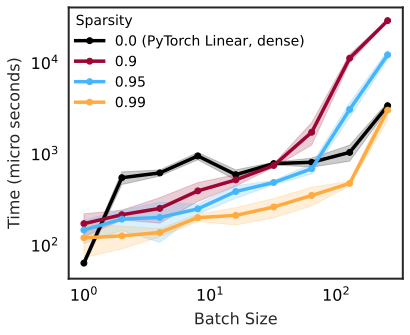
\includegraphics[width=\linewidth]{srigl_example_figs/CPU_benchmark.pdf}
        \caption{\textbf{PyTorch timings.} Benchmarking a naive (non-optimized) PyTorch implementation of our condensed  representation on CPU.}\label{fig:CPUbenchm}
    \end{minipage}
\end{figure}
\end{block}
\end{column}

\separatorcolumn

\begin{column}{\colwidth}

  \begin{block}{Neuron Ablation}
    \begin{itemize}
        \item At high sparsities, \gls{rigl} ablates large numbers of neurons. Effectively, \emph{\gls{rigl} reduces the width of the model at high sparsities}.
        \item Under a strict constant fan-in constraint, neurons can never be ablated. Leading to very sparely connected neurons at high sparsities.
        \item We implement a \textbf{neuron ablation method}, allowing \gls{srigl} to maintain both a constant fan-in constraint \emph{and} to reduce layer width at high sparsities.
    \end{itemize}

\begin{figure}
    \centering
    \includegraphics[width=\colwidth]{srigl_example_figs/ablationvsnoablation_wide.pdf}
     \caption{\textbf{Neuron ablation.} At sparsity levels over 90\%, \gls{rigl} learns to completely mask (ablate) a large number of neurons within each layer, effectively reducing layer width. Imposing a constant fan-in constraint requires all neurons to have the same number of (non-pruned) incoming weights and therefore inhibits ablation, which results in worse generalization performance than \gls{rigl}. Allowing \gls{srigl} to ablate neurons  restores \gls{rigl}-level performance.}\label{fig:ablationvsnoablation}
\end{figure}

\begin{figure}
    \begin{minipage}[t]{.48\colwidth}
        \includegraphics[width=0.49\colwidth]{srigl_example_figs/imagenet_perc_active.pdf}
        \caption{Neuron Ablation}\label{fig:imagenet_perc_active}
    \end{minipage}
    \hfill
    \begin{minipage}[t]{.48\colwidth}
        \includegraphics[width=0.48\colwidth]{srigl_example_figs/vit_rigl_fan_in.pdf}
        \caption{\textbf{Sparse Fan-In vs. \gls{vit} layer index at the end of training with \gls{rigl} at 90\% sparsity}. Only the first 10 layers are shown for clarity. We find that \gls{rigl} learns a sparse connectivity with large variance in fan-in between neurons within the same layer with some neurons receiving up to $\times 10$ the number of active connections than the mean for the same layer.}\label{fig:vit-rigl-fan-in}
    \end{minipage}
\end{figure}


  \end{block}

  \begin{block}{Acknowledgements}
  We acknowledge the support of the Natural Sciences and Engineering Research Council of Canada (NSERC), Alberta Innovates, the Digital Research Alliance of Canada, the NSF AI Institute for Artificial Intelligence and Fundamental Interactions (IAIFI). We are grateful for computational resources made available to us by Google and Denvr Dataworks. We also acknowledge the very helpful feedback of Trevor Gale. 

  \end{block}

  \begin{block}{References}

    % \nocite{*}
    \footnotesize{\bibliographystyle{icml2023}\bibliography{poster}}

  \end{block}

\end{column}

\separatorcolumn
\end{columns}
\end{frame}

\end{document}
